\documentclass[useAMS,usenatbib]{mn2e}

\usepackage{multicol}
\usepackage[english]{babel}
\usepackage{graphicx}
\usepackage{epsfig}
\usepackage{natbib}
\usepackage{times}
\usepackage{ulem}
\usepackage{array}
\usepackage[T1]{fontenc}
%\usepackage[section] {placeins}
\bibliographystyle{mn2e}
\citestyle{mn2e}


%%%%%%%% Begin custom definitions %%%%%%%%%%%%%
\usepackage{float}
\usepackage{caption}
\usepackage{amsmath}
\usepackage{amssymb}
\input macros.tex
\voffset=-1.4cm
\graphicspath{{./plots/}}
%%%%%%%% End custom definitions %%%%%%%%%%

\begin{document}

\title[Seed Black Holes in the First Galaxies]{The Dynamics of Seed
  Black Holes in the First Galaxies}

\author[C. Shi et al.]{Chao Shi$^1$\thanks{e-mail:
    cshi31@gatech.edu}, John H. Wise$^1$, Other authors\\
  $^{1}$ Center for Relativistic Astrophysics, Georgia Institute of
  Technology, 837 State Street, Atlanta, GA
  30332, USA\\
}
\pagerange{\pageref{firstpage}--\pageref{lastpage}} \pubyear{2015}

\maketitle
\label{firstpage}

\begin{abstract}

  \textbf{Copied from AAS.  Should be updated before submission with
    main results.} The discovery of bright quasars at redshift $z \ge
  6$ in the Sloan Digital Sky Survey implies that black holes (BHs) as
  massive as $10^9 \Ms$ were already assembled within 1
  Gyr. Generically, these SMBHs are thought to have assembled by
  mergers with other BHs and by gas accretion onto less massive seed
  BHs. One candidate of such seed BHs are Population III (Pop III)
  stellar remnants. In order to map out plausible scenarios such
  massive objects form from Pop III remnants, we run a cosmological
  adaptive refinement mesh simulation of an overdense region of about
  300 Mpc$^3$, which forms a few $10^9 \Ms$ dark matter halos and over
  13000 Pop III stars by redshift 15. Then we focus on one of these
  massive halos, containing 20 Pop III stellar remnants, to study the
  dynamical behavior of these BH seed candidates. Here we report on
  the evolution of the orbital properties of stellar-mass seed BHs in
  one of the first galaxies. They are distributed throughout the halo,
  creating a swarm of BHs, gradually falling toward the halo center
  through dynamical friction. From these characteristics, we estimate
  the BH merger rate in this particular galaxy, which is an important
  quantity to assess during the early buildup of massive BHs.

\end{abstract}

\begin{keywords}
  galaxies: formation -- galaxies: dwarf -- galaxies: high-redshift --
  methods: numerical
\end{keywords}

\section{Motivation}
% why study SMBH? Especially, why DYNAMICS?
Since the discovery of bright quasars by Sloan Digital Sky Survey(SDSS) at high
redshift(\textit{z}$\gtrsim$6), accretion onto super massive black holes(SMBHs) in the center
(Fan et al 2006) is believed to be the only feasible power supply for some of 
the most luminous objects. If the accretion is at or below Eddington rate, the
black holes must be as massive as $10^9\mbox{M}_{\odot}$(Willott et al. 2003),
which indicates that such massive objects were in place already when the
universe was less than one billion years old. How such massive BHs formed within
such a short period of time is still an open question. They must form early on
and grow very rapidly through accretion and/or merger(Haiman\&Loeb 2001). Simple
estimation shows that if the
``seed'' BH has an inital mass of $1\mbox{M}_{\odot}$, it has to accrete at or
above Eddington rate during its entire lifetime(Volonteri\&Bellovary 2012). 
Given feedback effects must exist to power the quasar, this scenario is extrmely
unlikely, if not impossible. It will be more favorable if the seed BHs have an
``intermediate'' intial mass, e.g. between $100\ -\ 10^5\mbox{M}_\odot$
(Volonteri\&Bellovary 2012). The remnants of the very first generation of
stars(Pop III stars), is considered as a promising candidate that falls in this
category(Madau \& Rees 2001). \\

% other work that has already studied these
(More references to be filled in here to summarize other work down this
line\dots)
% mention Haiman's paper, which is semi-analytical. \\

% our work
% we did a full numerical study. \\
It is then natural to investigate the formation of seed BHs from Pop III
remnants in a fully cosmological background, which is the emphasis of this
paper. We first do a stacked analysis on a cosmological simulation
presented in Xu et al.(2013), which has relatively large survey volume, for
spatial distribution and orbital properties of seed BHs candidates. Then we run
a zoom-in simulation based on the previous simulation for a high temporal
analysis focusing on one single massive halo. In order to estimate seed BHs
merger rate in first galaxies, we also perform a simulation with the same
physics, much higher output frequency(1000 data sets) and thus smaller survey
volume ( ($1\mbox{Mpc})^3$ ) due to limited computational power. 
\section{Methods}
Physics module description to be filled in here\dots
\subsection{Simulation Setup}
Our analysis starts from the ``Rarepeak'' simulation conducted by Xu et al.
(2013) that focuses on the frist stars and galaxies in an overdense region with 
$\langle\delta\rangle \equiv \langle\rho\rangle/(\Omega_M\rho_c)-1\simeq 0.65$
at $z=15$ in the volume of 135 comoving $\mbox{Mpc}^3$, where $\Omega_M$ is the density
of matter in units of critical density $\rho_c = 3H^2_0/8\pi G$. The simulation
is performed with the adaptive mesh refinement(AMR) cosmological hydrodynamics
code \textit{Enzo} (Bryan et al. 2014). Radiation transport of ionizing photons are
tracked by the adaptive ray tracing module \textit{Moray}, which is coupled to the
hydrodynamics, energy and chemistry solvers in \textit{Enzo}. We have studied the
number of Pop III remnants in the first galaxies(Xu et al. 2013), their
contribution to the X-ray background(Xu et al. 2014). In this paper, we focus on
the evolution of seed black holes(BHs) formed from these Pop III remnants. 
Here we give an overview of the simulation setup and numerical methods. A more 
detailed description of the star formation and feedback models are given in 
Wise et al. (2012a, 2012b) and Xu et al.(2013).\\

MUSIC(Hahn\&Abel 2011) is used to generate the initial condition for the
simulation at $z=99$. The cosmological parameters are adopted from the 7-year
\textit{Wilkinson Microwave Anisotropy Probe}(WMAP) $\Lambda\mbox{CDM}$+SZ+LENS
best fit (Komatsu et al. 2011):$\Omega_M=0.266, \ \Omega_{\Lambda}=0.734,\
\Omega_b=0.0449,\ h = 0.71,\ \sigma_8=0.81,\ \mbox{and}\ n=0.963$, where the
variables have the usual definitions. We use a comoving simulation volume of
$(40\mbox{Mpc})^3$ that has a $512^2$ root grid resolution and three initial
nested grids each with mass resolution eight times higher in each nested grid,
which corresponds to an effective inital resolution of $4096^3$ and dark
matter(DM) mass resolution of $2.9\times 10^4\mbox{M}_{\odot}$. The
comoving voulme of a finest nested grid is $5.2\times 7.0 \times 8.3\ 
\mbox{Mpc}^3(302\ \mbox{Mpc}^3)$. Further refinement in the Lagrangian volume of
the finest nested grid is allowed up to a maximum AMR level $l = 12$, giving a
maximal spatial resolution of 19 comoving pc. Refinement occurred when either a
baryon or DM overdensity of $4\times\Omega_{\{\textrm{b,DM\}}}\rho_cN^{l(1+\phi)}$
, where $N=2$ is the refinement factor , and $\phi=-0.1$ allows more aggressive
refinement at higher densities, i.e., super-Lagrangian behavior. At $z=15$
where the simulation ends, we have a large number (~1000) of halos with
$M>10^8\mbox{M}_\odot$, three of which with $M>10^9\mbox{M}_\odot$, in the
Lagrangian region with a comoving volume of 
$3.8\times5.4\times6.6\mbox{Mpc}^3(135\mbox{Mpc}^3)$. \\
At this point, new formation of Pop III stars delines rapidly while the
formation rate metal-enriched stars continues to increase. Pop III and
metal-enriched stars have different formation and feedback models, distinguished
by the total metallicity of the densest star-forming cell. The former are formed
if [Z/H] < -4, and the latter are formed otherwise. The star formation and
feedback models are the same as the ``RP'' simulation in Wise et al.(2012a),
except that the characteristic mass $M_{char} = 40\mbox{M}_{\odot}$ of the Pop
III inital mass function(IMF), whereas Wise et al. used $100\mbox{M}_{\odot}$.
The Pop III stellar masses are randomly sampled from an IMF
\begin{gather}
  f(\log M)dM =
  M^{-1.4}\exp\left[-\left(\frac{M_{char}}{M}\right)^{1.6}\right]dM
\end{gather}
that behaves as a power-law IMF at $M > M_{char}$ and is cutoff exponentially
below that mass(Chabrier 2003). Latest results of Pop III stars formation
simulation shows that choosing $M_{char}$ this way is more consistent(e.g. Turk
et al. 2009; Greif et al. 2011; Hriano et al. 2013; Susa 2013; Susa 2014).
Metal-enriched star formation is modeled as in Wise \& Cen(2009), which is
similar to the Pop III prescription without the requirement of minimum
$\mbox{H}_2$ fraction. This requirement is not valid in this case because the
metal-enriched gas can efficiently cool even in the presence of a strong UV
radiation field(e.g. Safranek-Shrader et al. 2010). Star formation is restricted
to cold gas, with temperatures $T < 1000 K$. Pop III star particles represent
individual stars, whereas metal-enriched star particles represent a star cluster
of some total mass and an presumed normal (i.e., Kroupa) IMF minimum and maximum
stellar masses inferred in the Milky Way. The minimum mass of a star particle is
set to $m_{\star,min} = 1000 \mbox{M}_{\odot}$. The star particle does not
provide any and continues to accrete until it reaches $m_{\star,min}$.

%Further zoom-in simulation description

%John's simulation on Bluewater(for more representative massive halos)
\subsection{Orbital Elements}
*approximation: key orbital properties of seed BHs: semi-major axes and
eccentricities\\
*calculation of semi-major axis and eccentricities\\
*Angular momentum and estimation of merger rate by the evolution.\\

\section{Results}

\subsection{Stacked Analysis}
Radial distribution of seed BHs at different stages:
%\begin{minipage}{\linewidth}
%\makebox[\linewidth]{ 
%  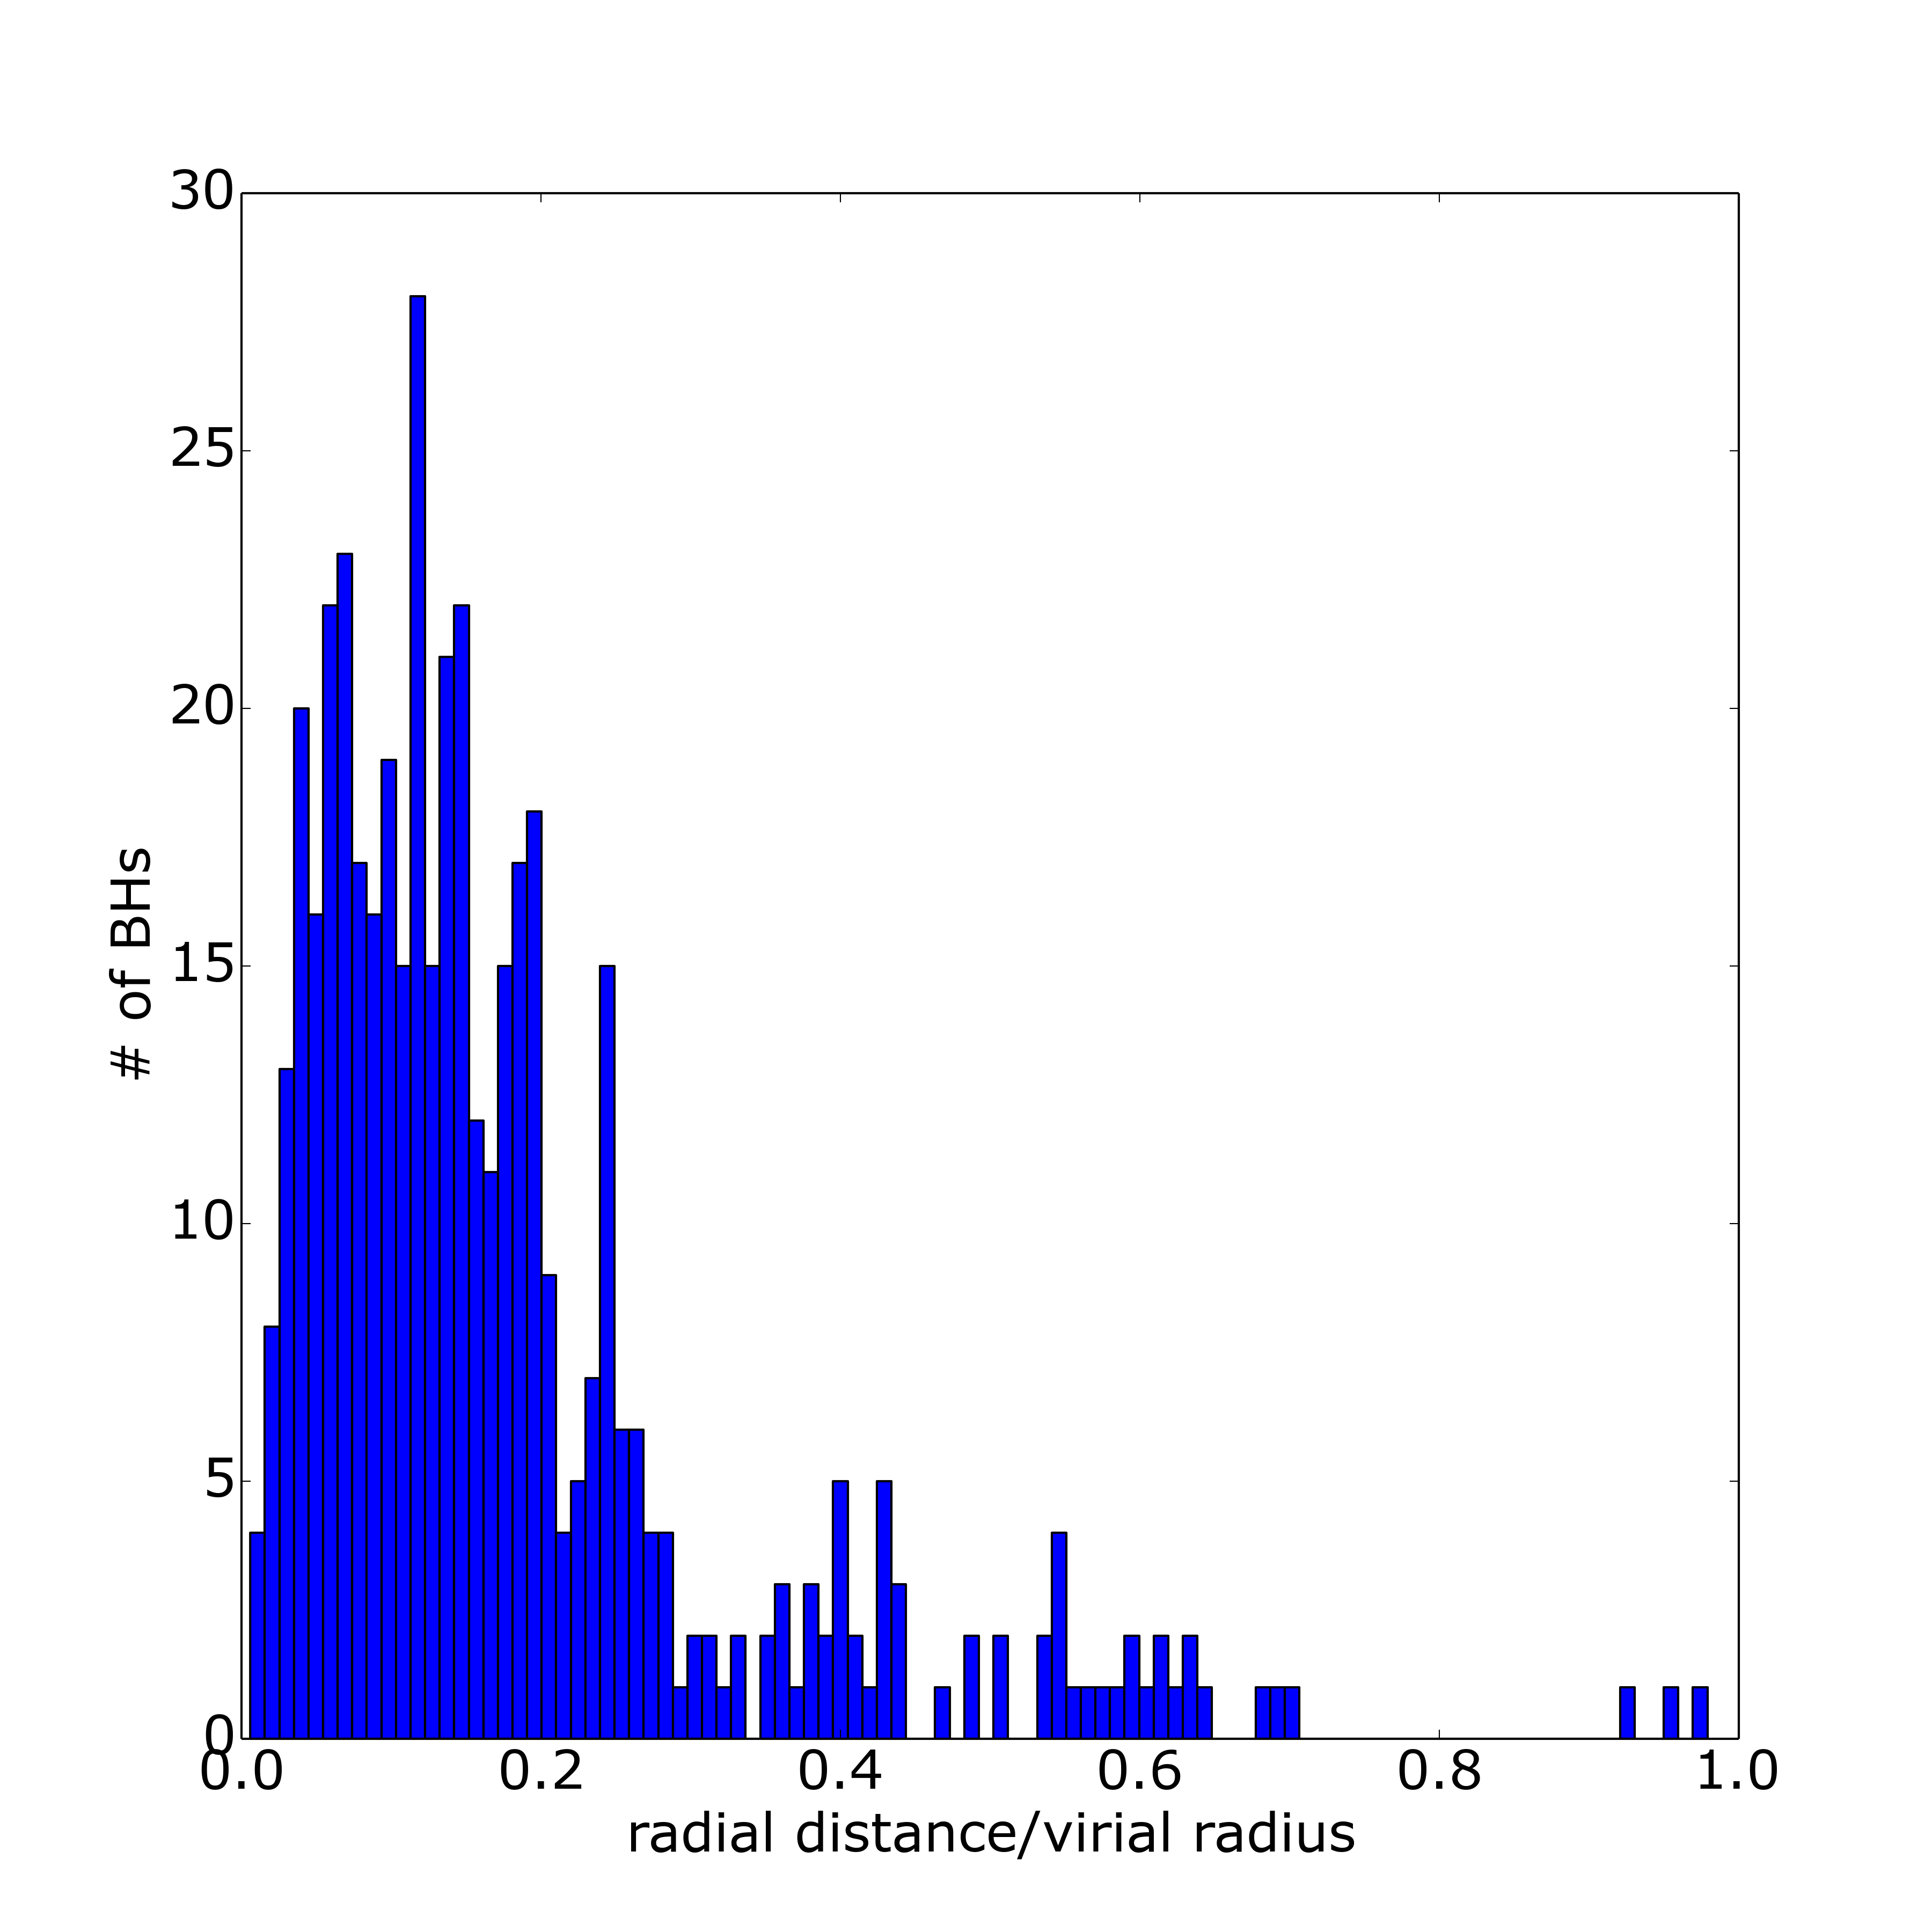
\includegraphics[keepaspectratio=true,width=0.8\linewidth]{rad_dist3.png}
%}
%\end{minipage}
%\begin{figure}
%  \centering
%  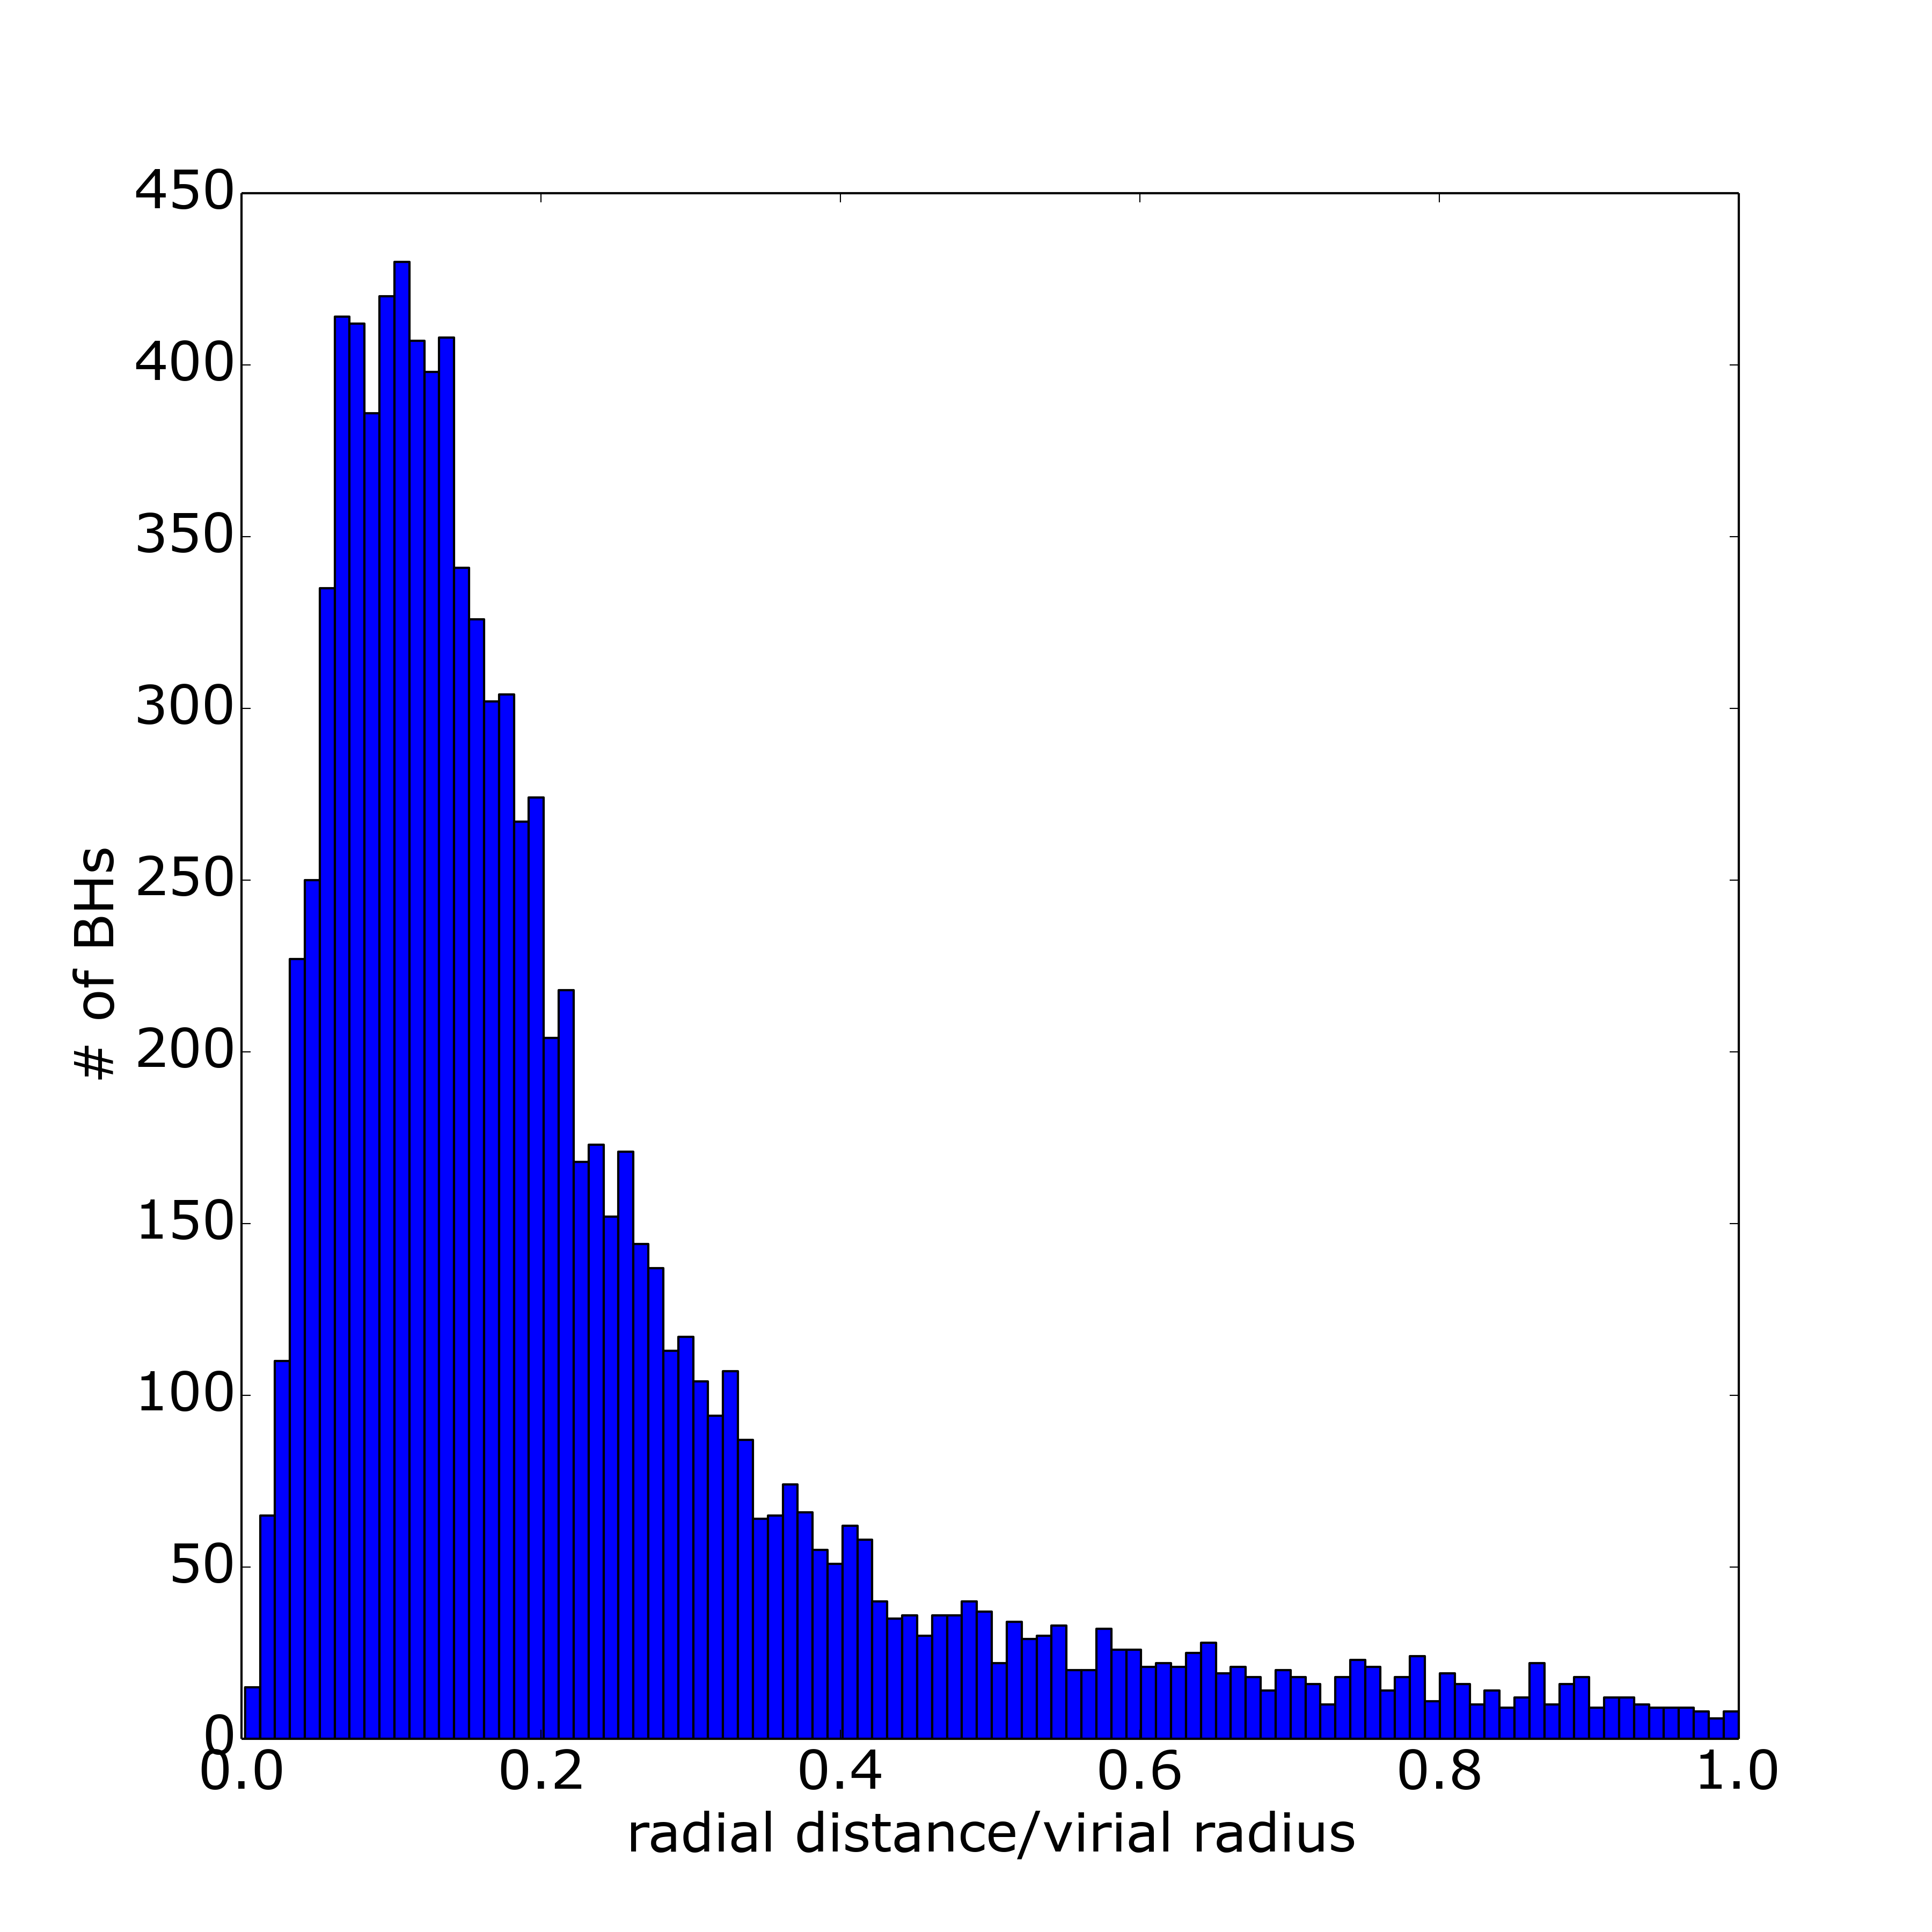
\includegraphics[width=0.8\columnwidth]{rad_dist14.png}
%\end{figure}
%\begin{figure}
%  \centering
%  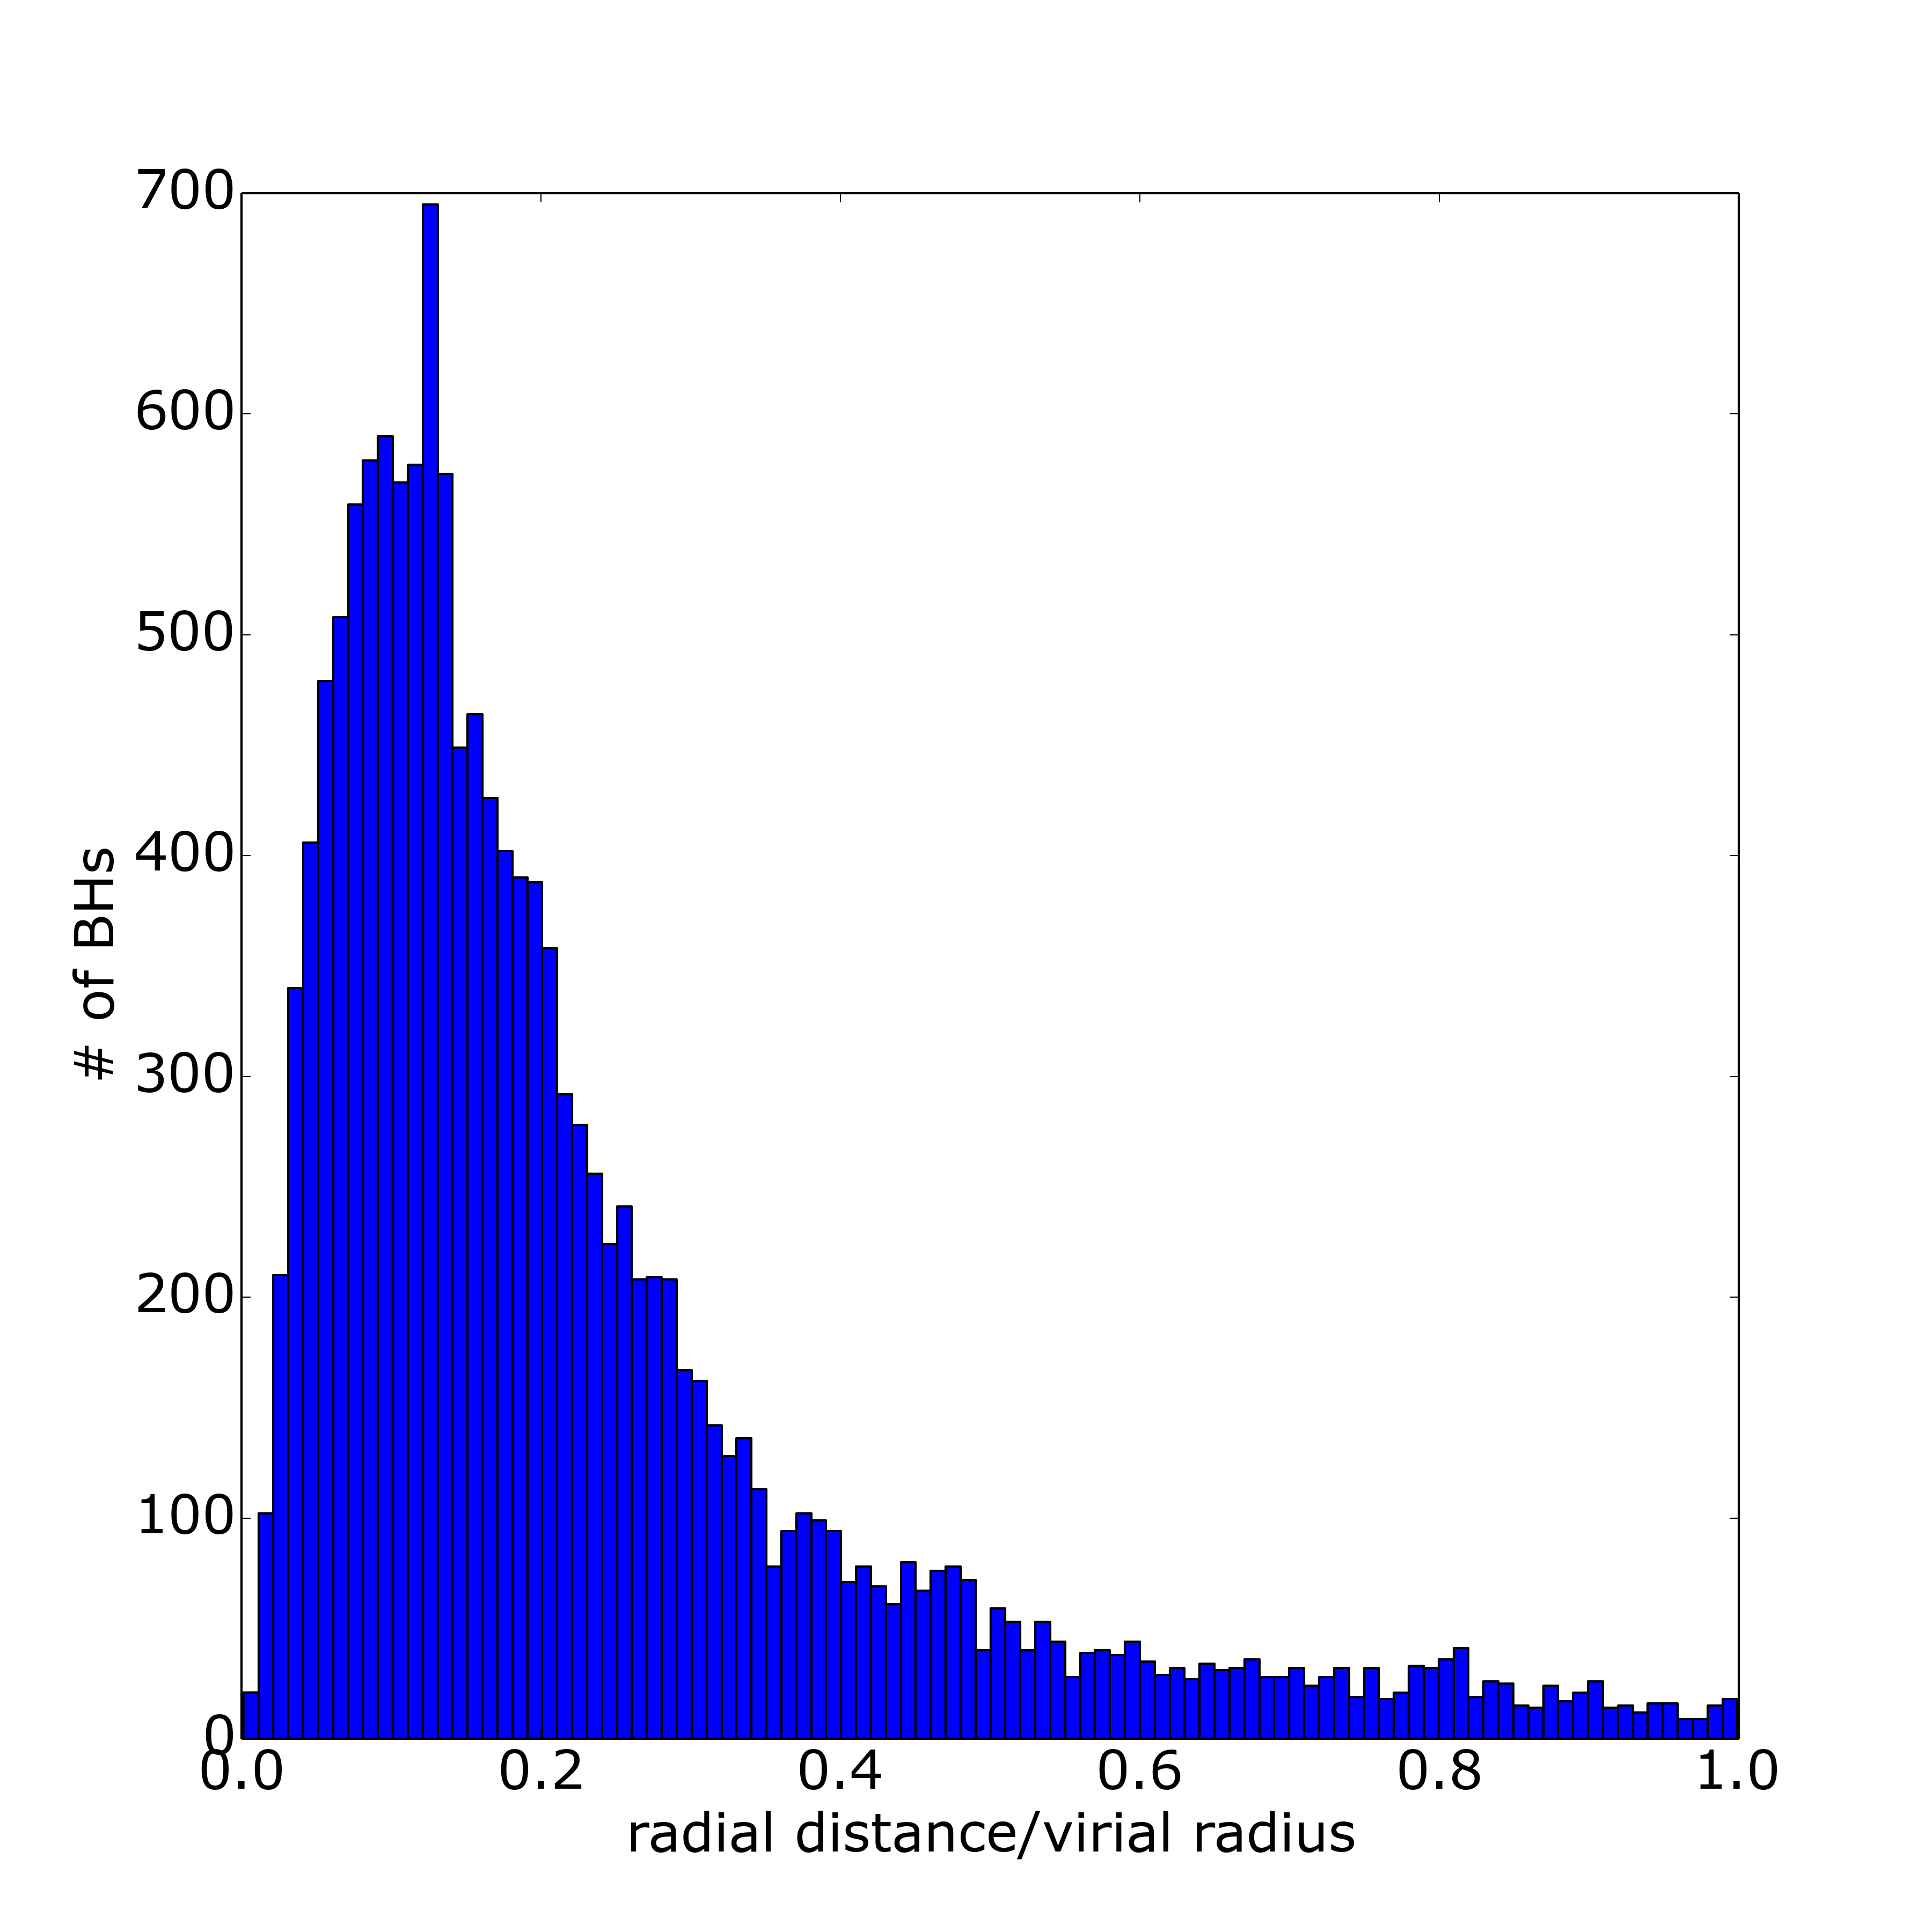
\includegraphics[width=0.8\columnwidth]{rad_dist22.png}
%\end{figure}
%Radial distribution of seed BHs of the final time step in different mass ranges:
%\begin{figure}
%  \centering
%  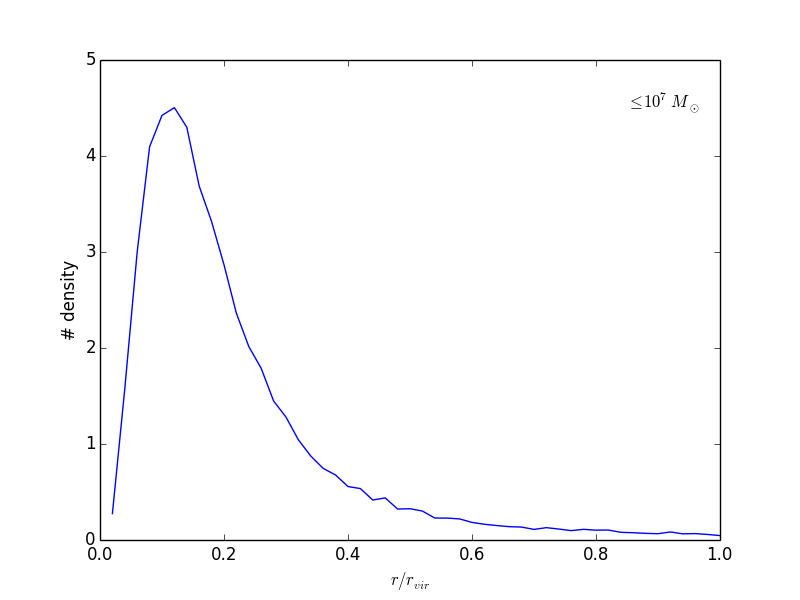
\includegraphics[width=0.8\columnwidth]{radist_mass7.png}
%\end{figure}
%
%\begin{figure}
%  \centering
%  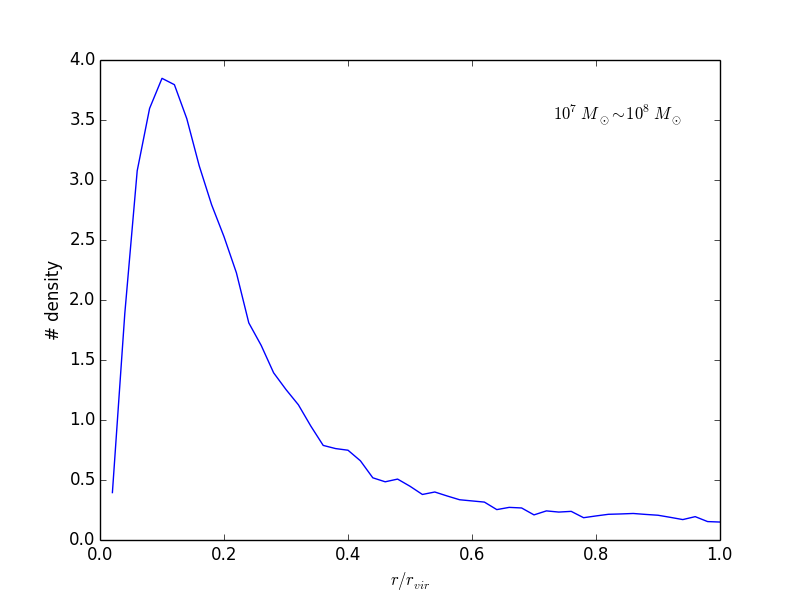
\includegraphics[width=0.8\columnwidth]{radist_mass8.png}
%\end{figure}
%
%\begin{figure}
%  \centering
%  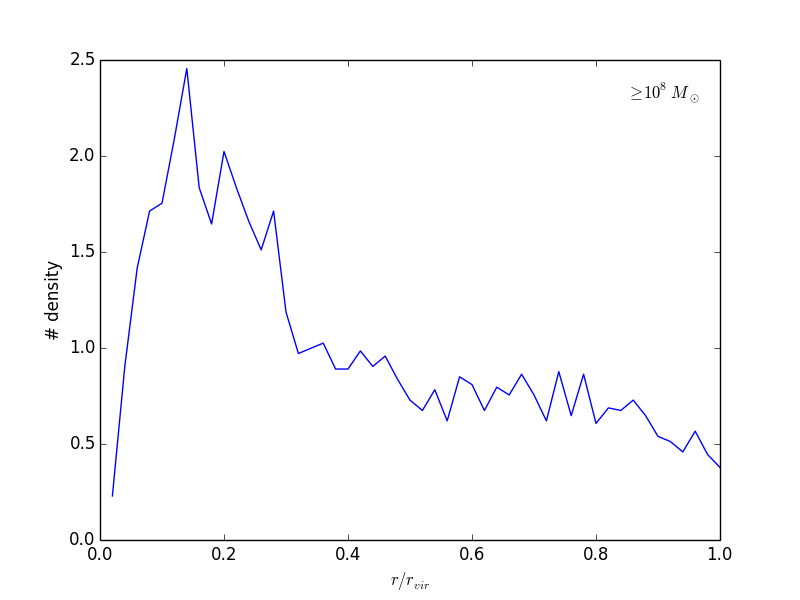
\includegraphics[width=0.8\columnwidth]{radist_mass9.png}
%\end{figure}

Orbital properties:
%\begin{figure}
%  \centering
%  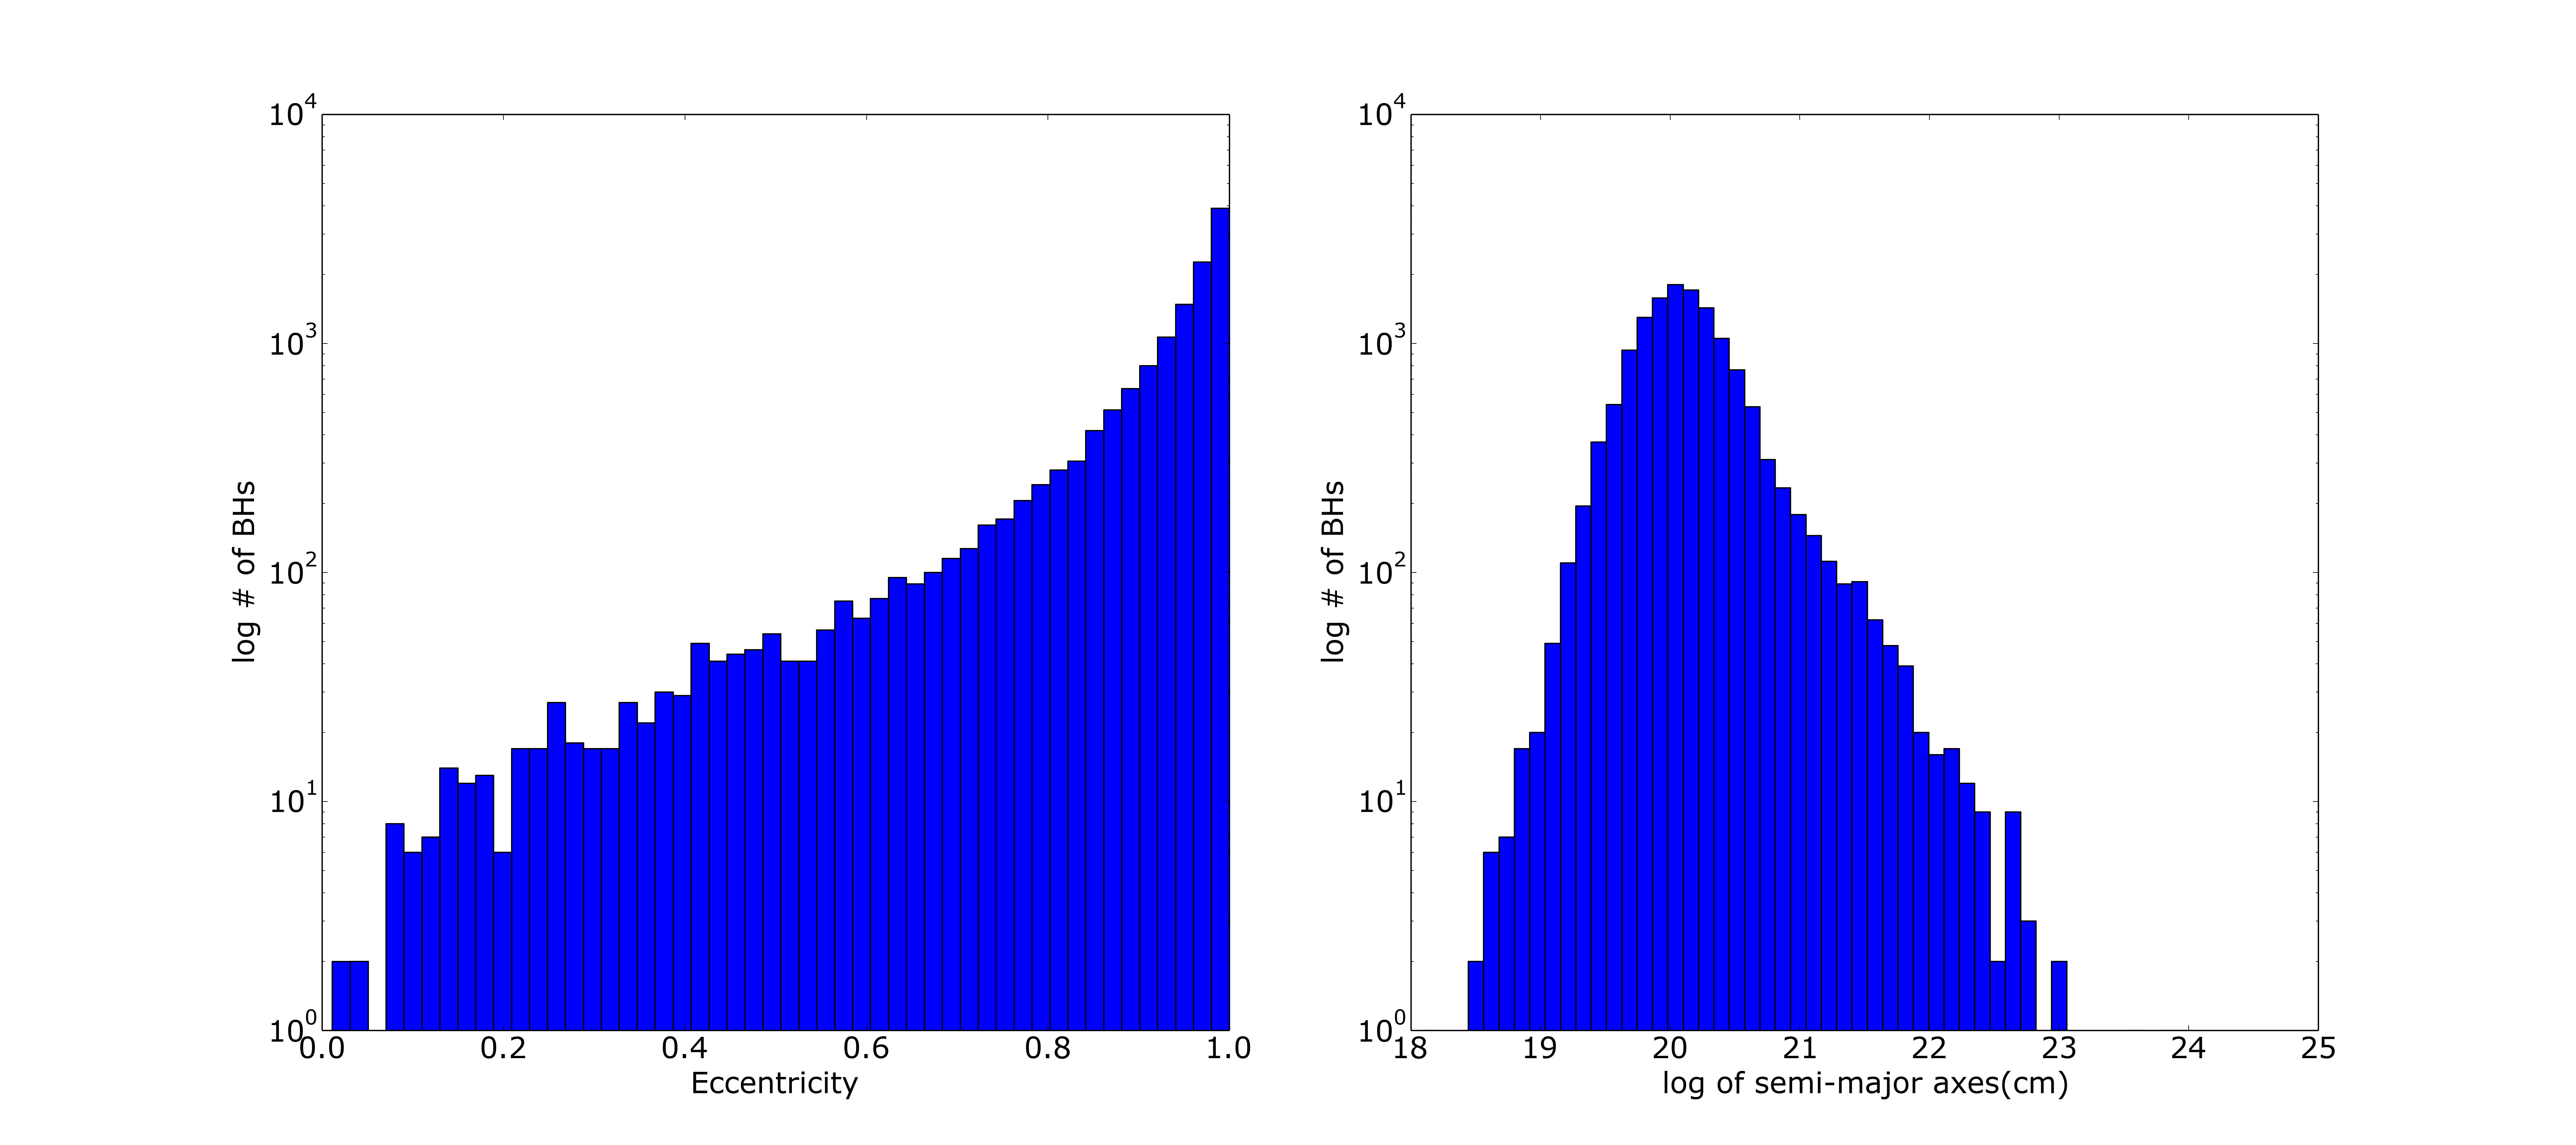
\includegraphics[width=0.8\columnwidth]{bhsorb_new.png}
%\end{figure}
%


\subsection{Case Study: High Temporal Analysis of a Single Galaxy}

Seed BHs position:
%\begin{figure}
%  \centering
%  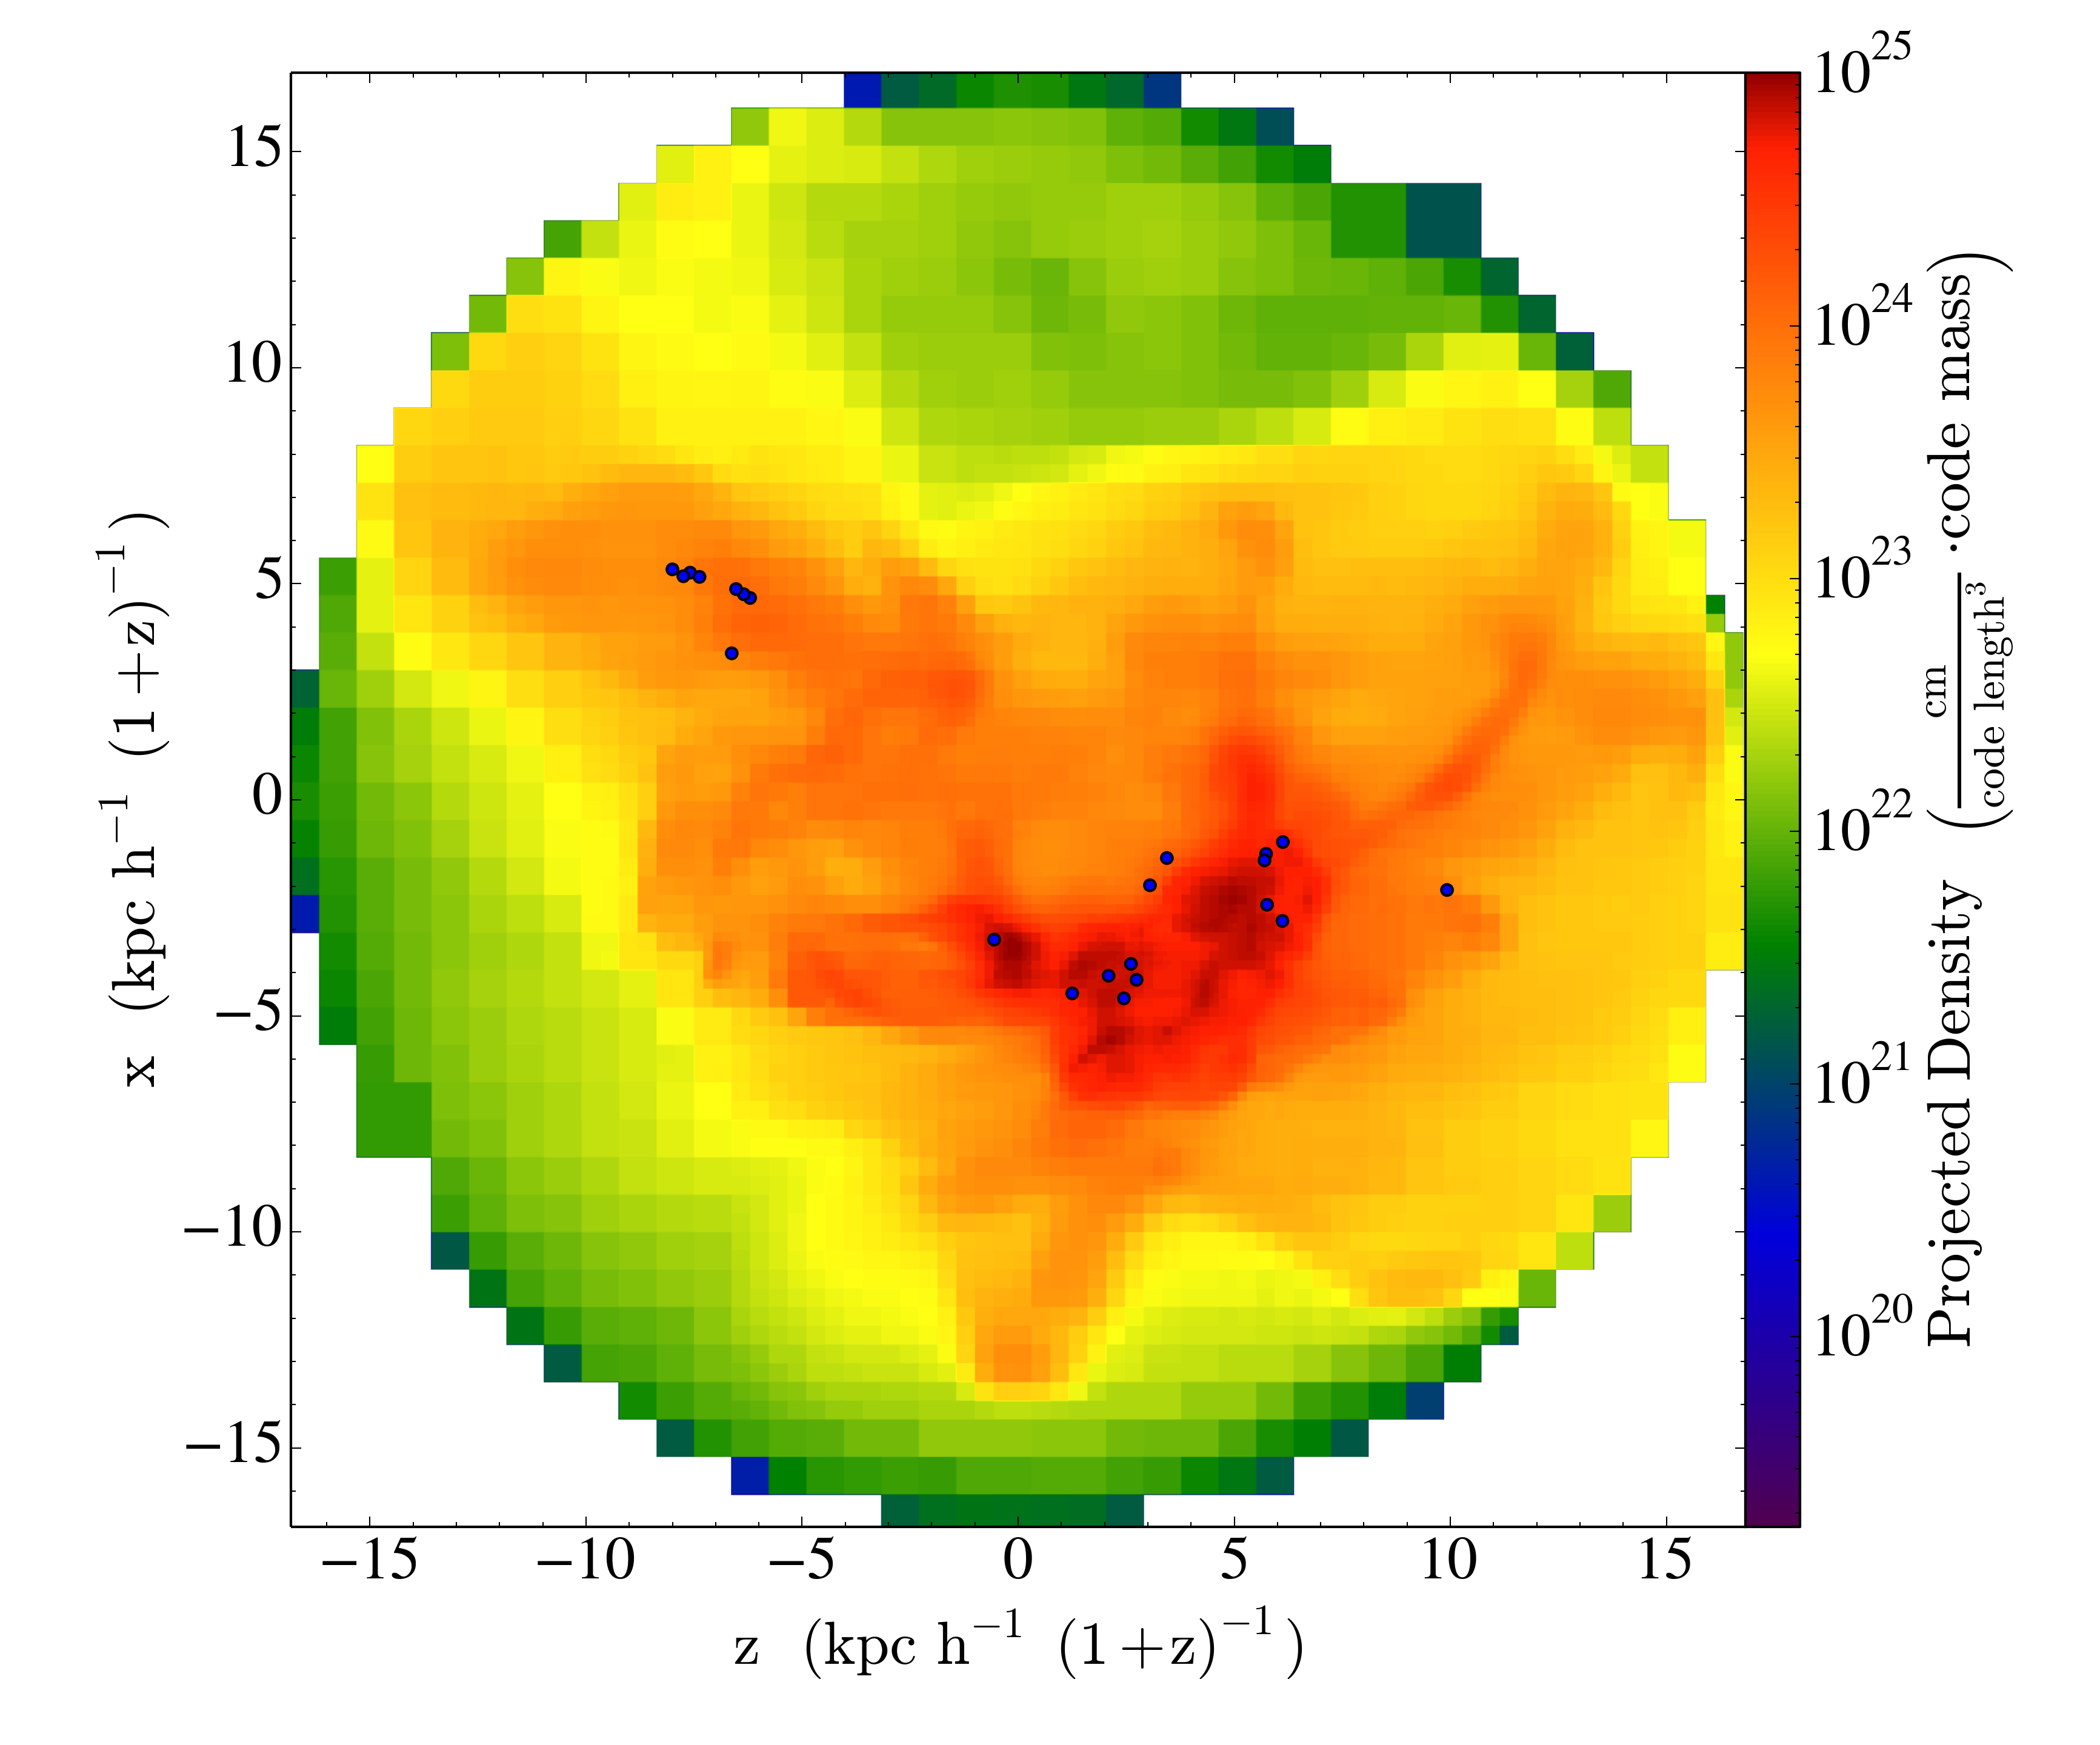
\includegraphics[width=0.8\columnwidth]{P0173_y_D.png}
%\end{figure}
%
%\begin{figure}
%  \centering
%  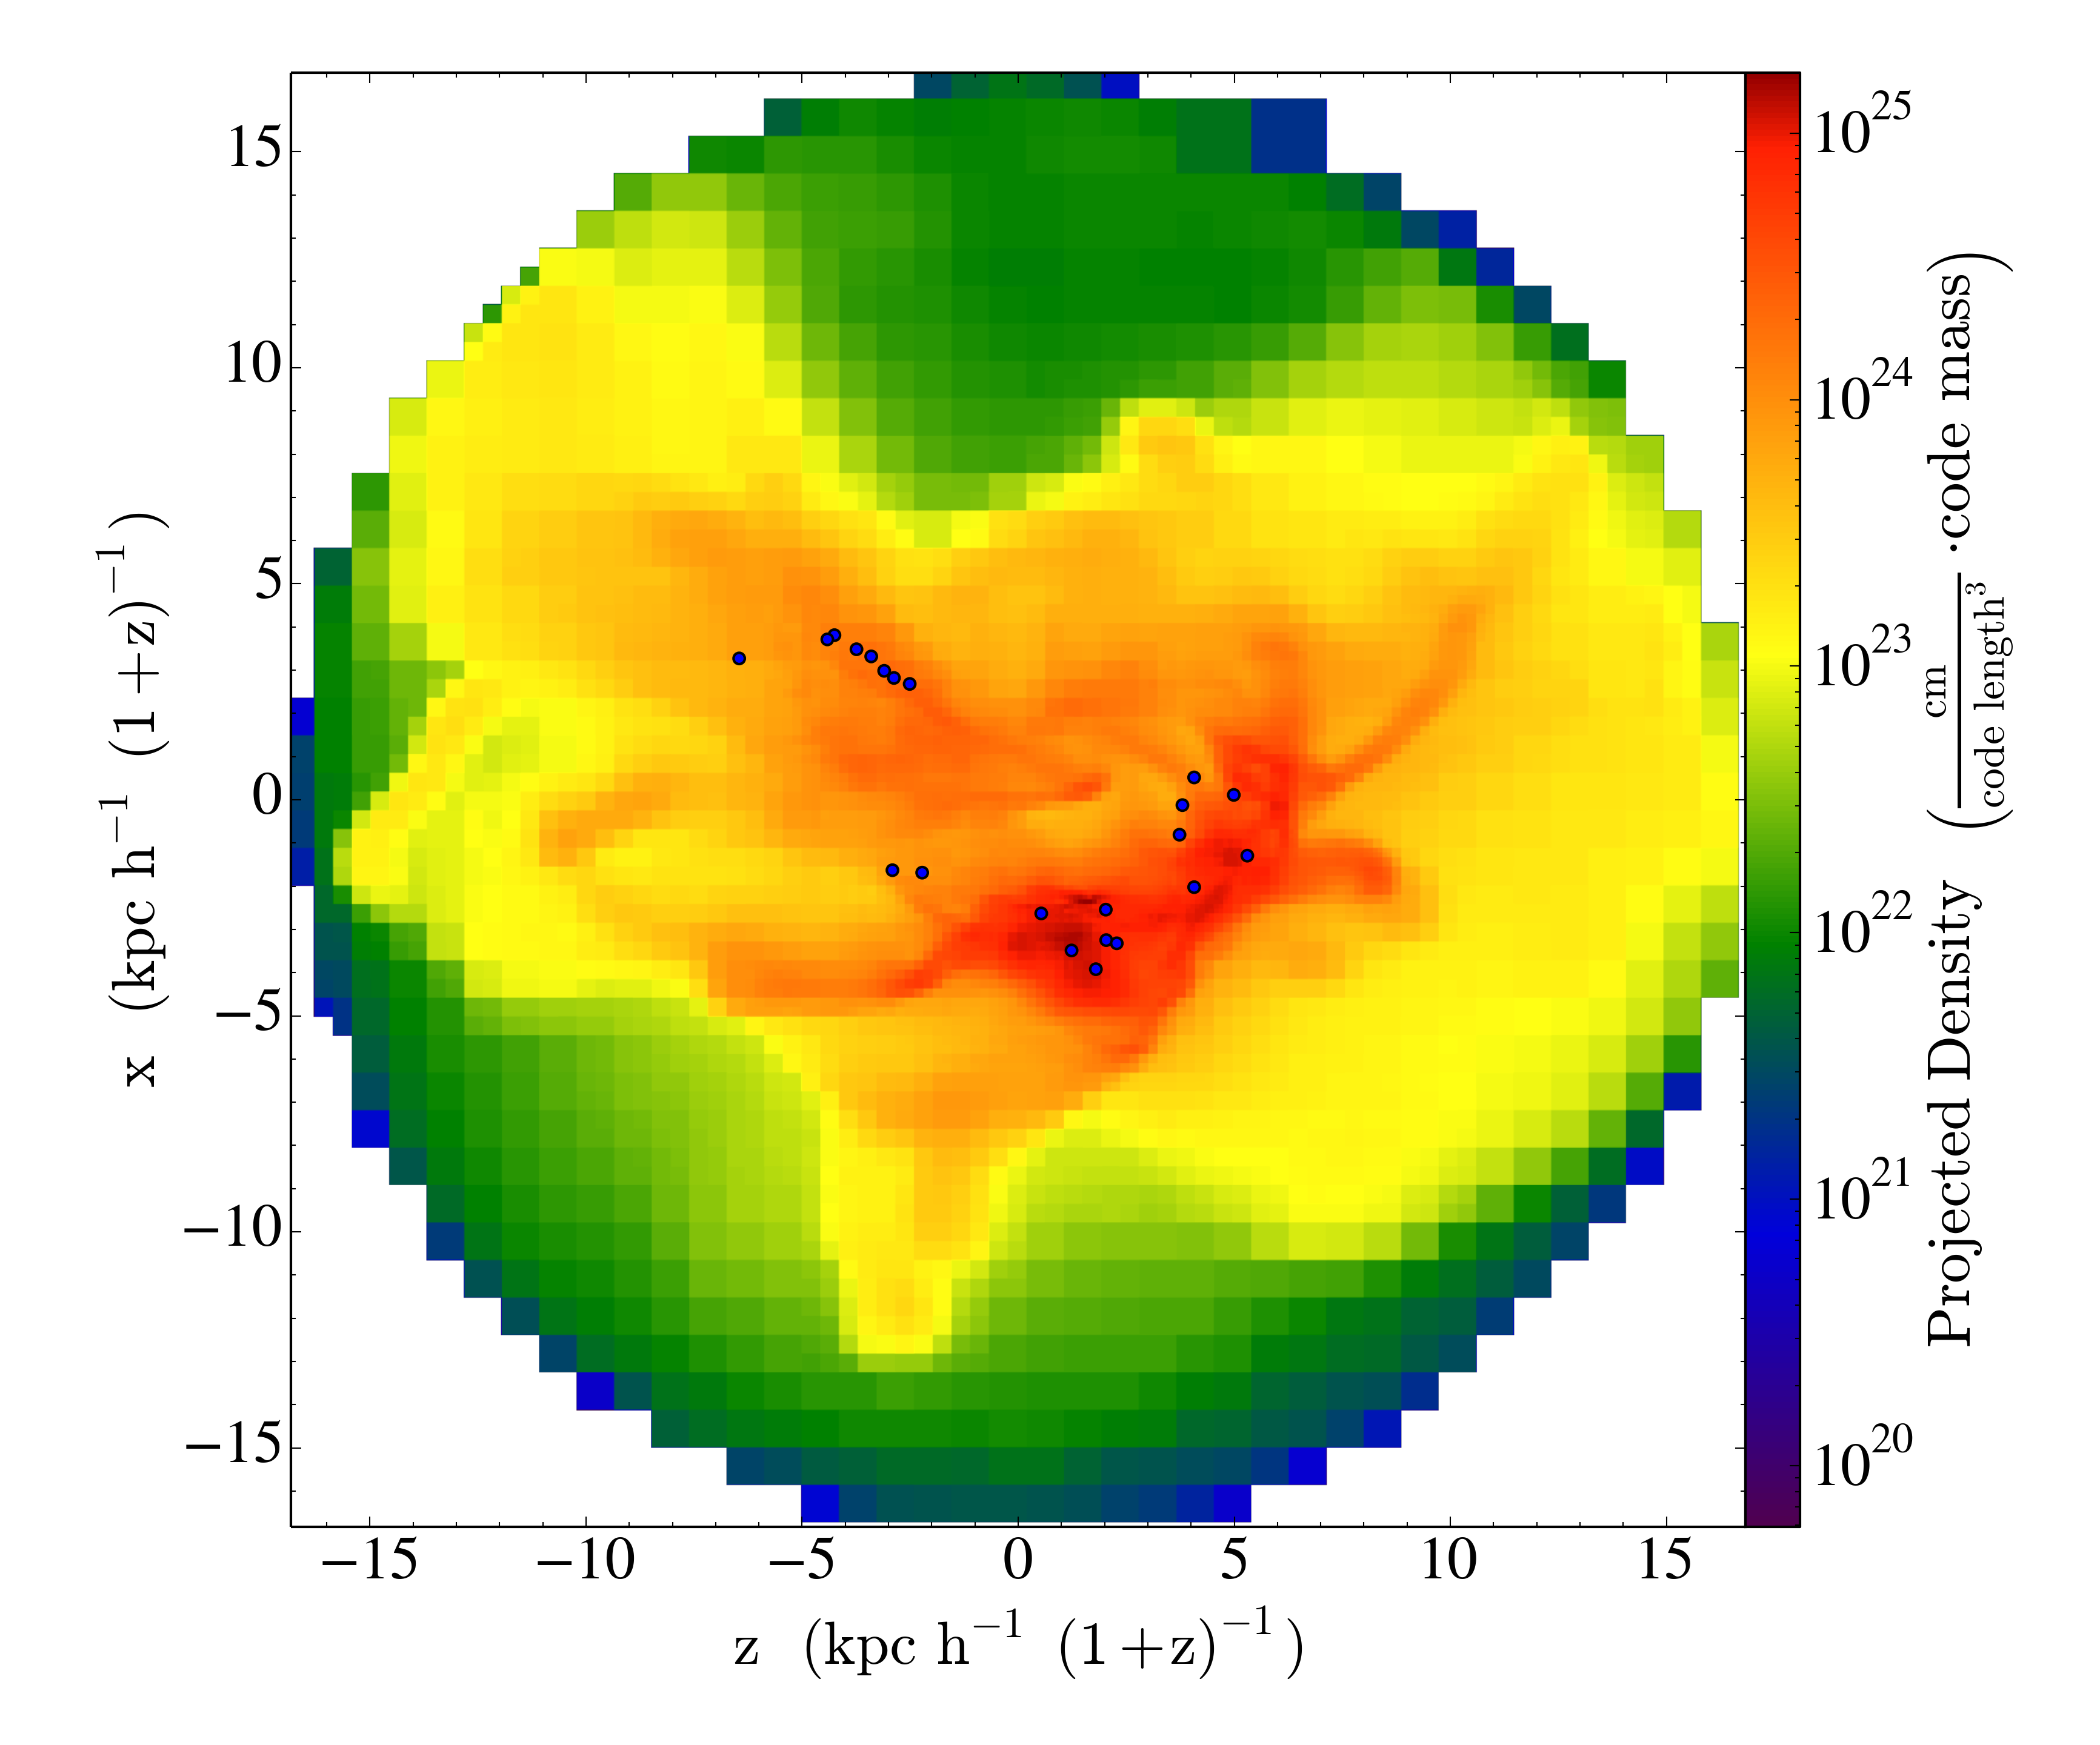
\includegraphics[width=0.8\columnwidth]{P0224_y_D.png}
%\end{figure}
%
%\begin{figure}
%  \centering
%  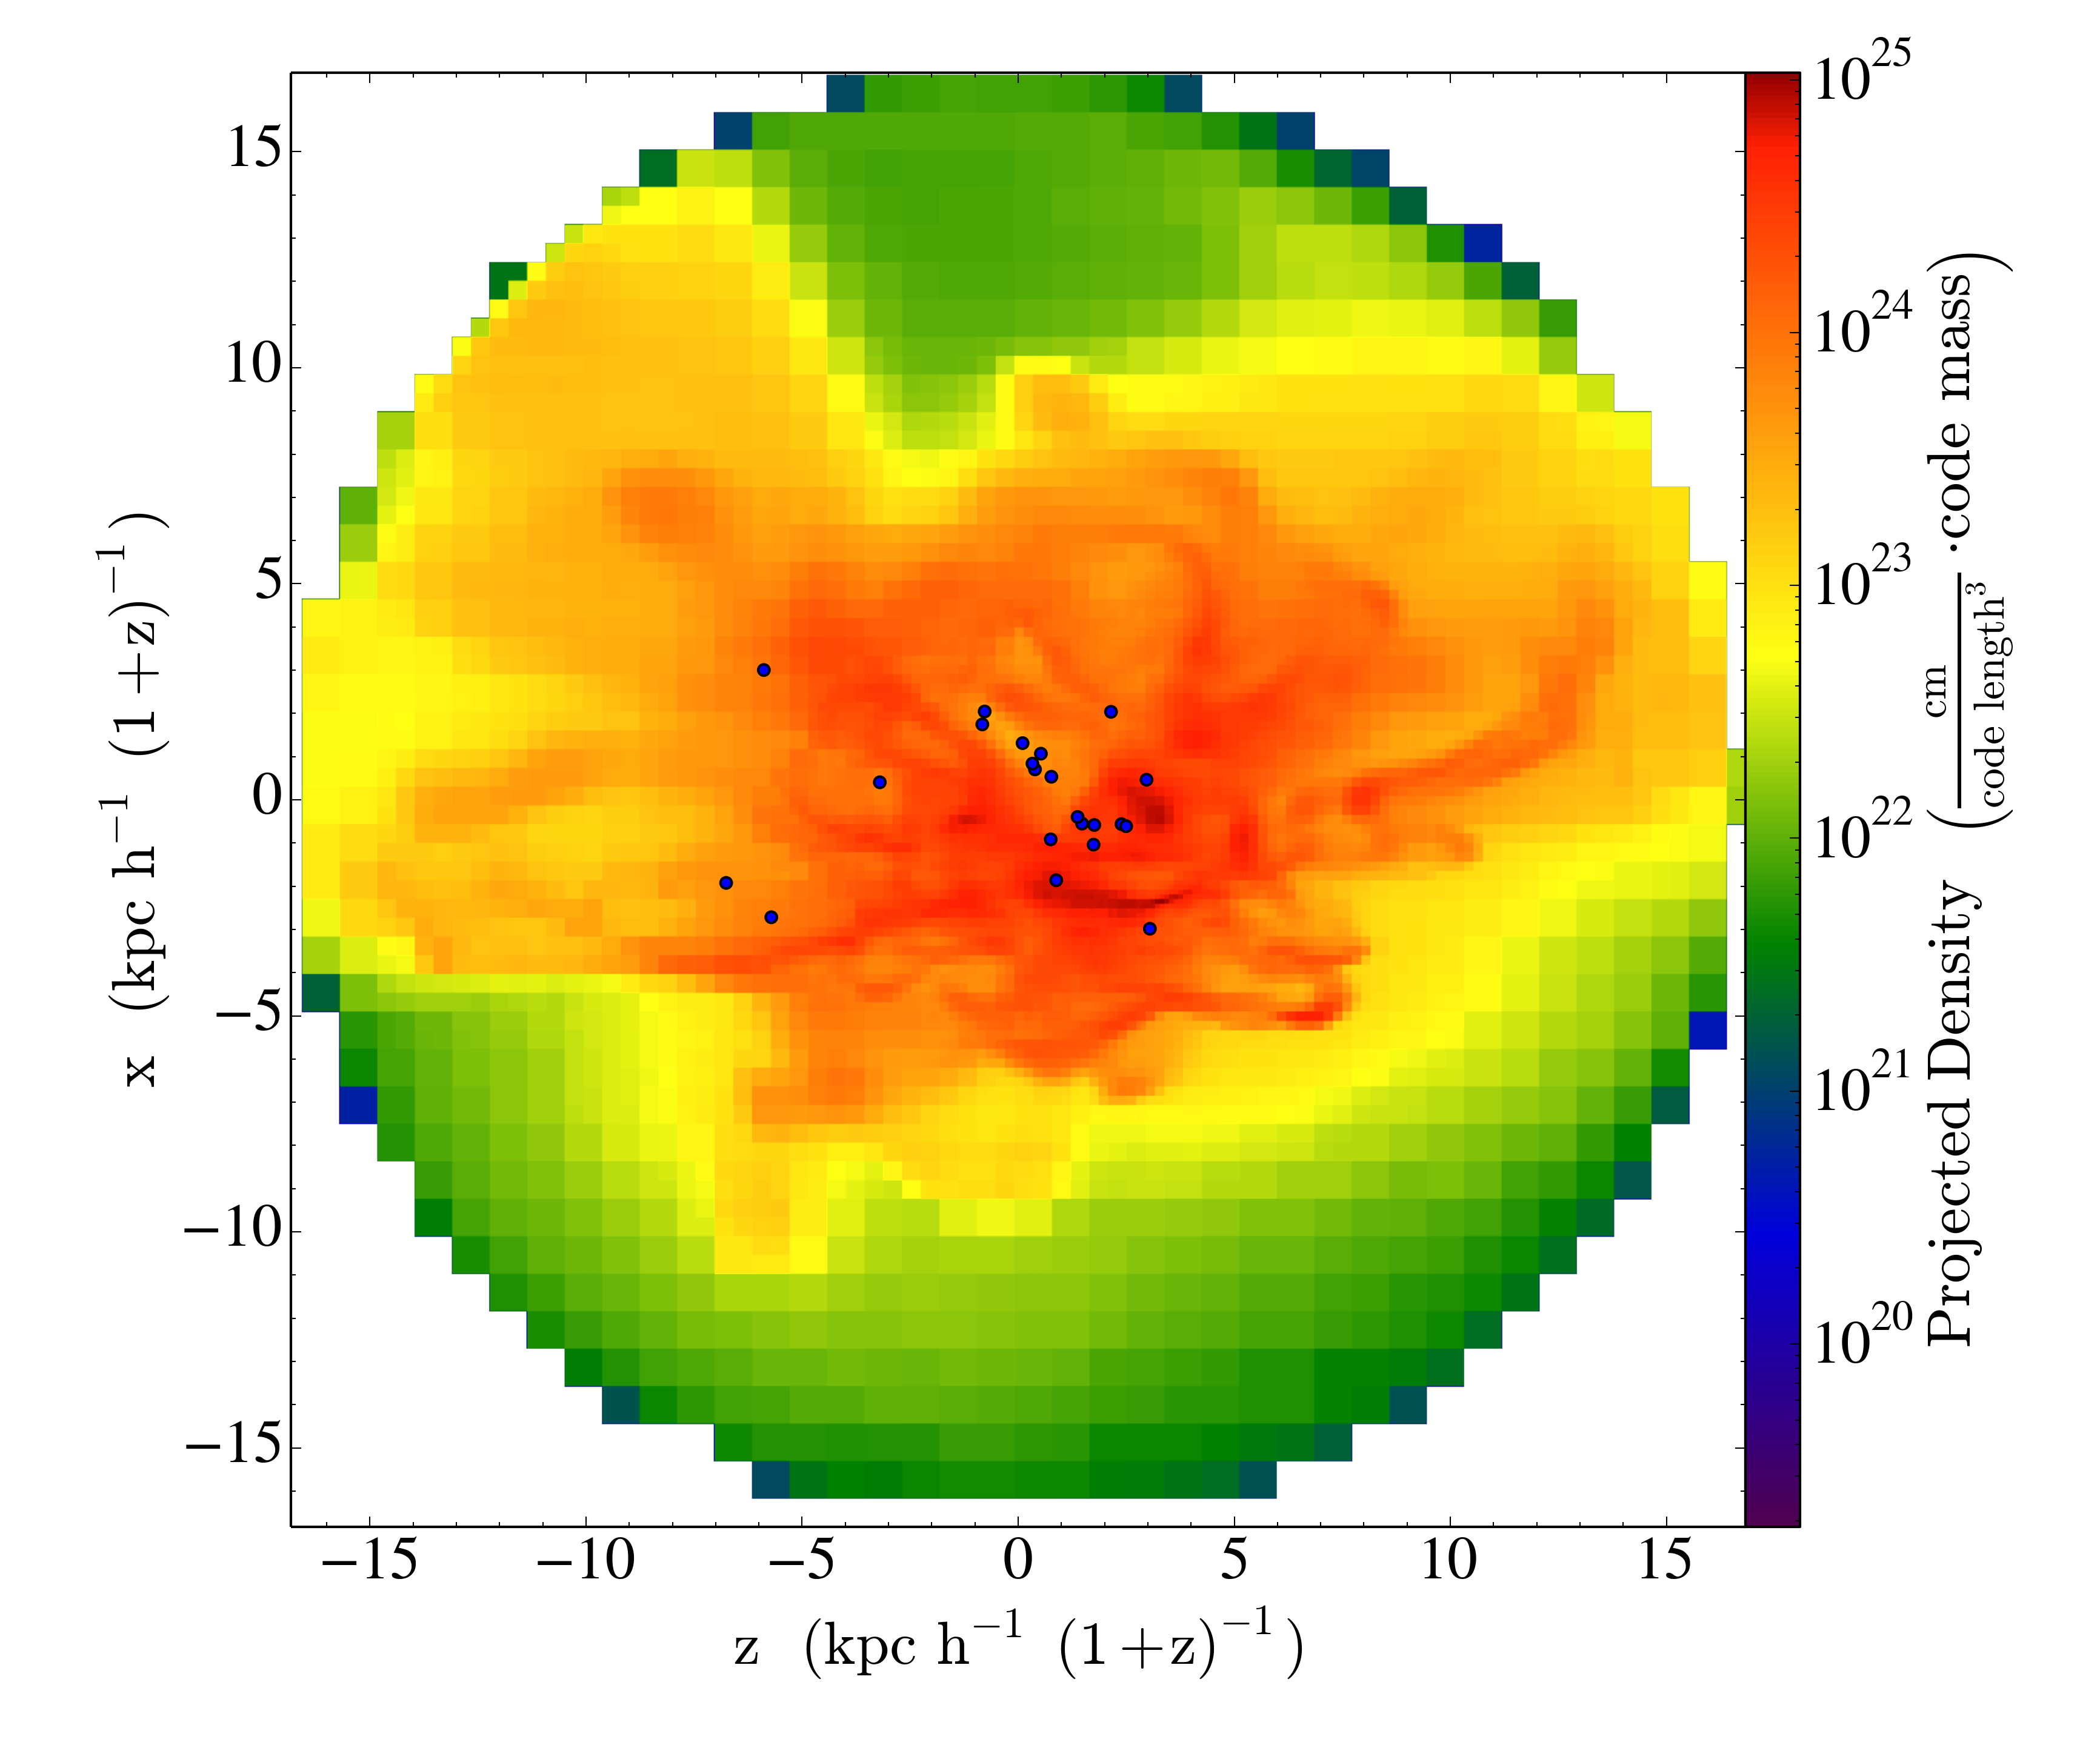
\includegraphics[width=0.8\columnwidth]{P0274_y_D.png}
%\end{figure}
Angular momentum evolution:

%\begin{figure}
%  \centering
%  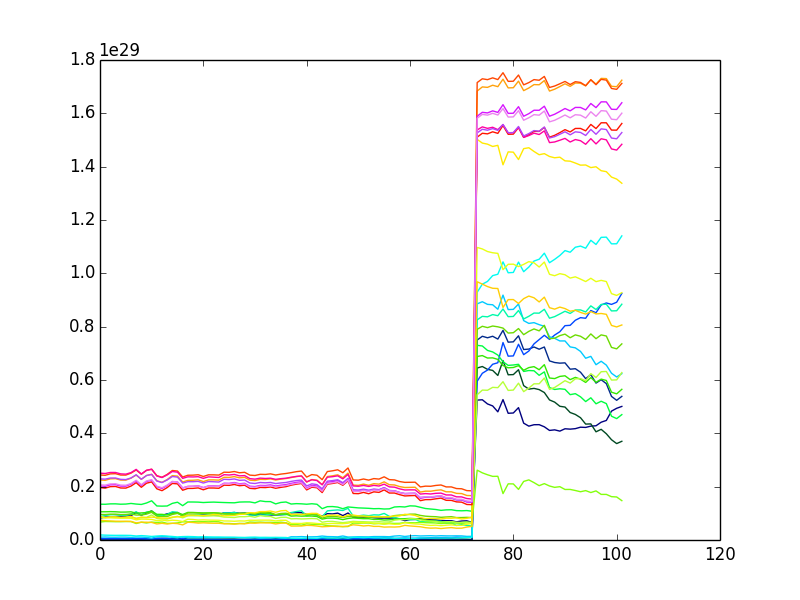
\includegraphics[width=0.8\columnwidth]{L2.png}
%\end{figure}


\section*{Acknowledgments}

This work is supported by NSF grants AST-1211626 and AST-1333360.
This research has made use of NASA's Astrophysics Data System
Bibliographic Services.  The majority of the analysis and plots were
done with \yt \citep{yt_full_paper}.

\bibliography{jwise}
\bsp
\label{lastpage}

\end{document}
